\documentclass[a4paper,11pt]{article}

	%% From https://github.com/aytchell/latex-listings-protobuf/tree/09c39676e6afb2af8c7d21ed21a516359c52e27c/

\usepackage{xcolor}
\usepackage{xcolor-solarized}
\usepackage{textcomp}

\newcommand{\SetProtoColorsSolarized}{
  % Colors taken from the 'solarized' color scheme of Ethan Schoonover
  % (with light background)
  % http://ethanschoonover.com/solarized
  \colorlet{proto_basic}{solarized-base00}
  \colorlet{proto_keyword}{solarized-cyan}
  \colorlet{proto_type}{solarized-cyan}
  \colorlet{proto_options}{solarized-cyan}
  \colorlet{proto_comment}{solarized-base1}
  \colorlet{proto_string}{solarized-blue}
  \colorlet{proto_number}{solarized-violet}
  \colorlet{proto_ident}{solarized-base00}
  \colorlet{proto_digits}{solarized-violet}
  \colorlet{proto_background}{solarized-base3}
}

\newcommand{\SetProtoColorsBlueish}{
  % Colors inspired by the NASM style of Robin Eklind
  % https://github.com/mewspring/latex
  \definecolor{proto_basic}{RGB}{0,0,0}             % black
  \definecolor{proto_keyword}{RGB}{0,0,0}         % black
  \definecolor{proto_ident}{RGB}{128,0,0}            % dark red
  \definecolor{proto_options}{RGB}{128,0,128}       % purple
  \definecolor{proto_comment}{RGB}{0,128,0}         % dark green
  \definecolor{proto_string}{RGB}{255,0,0}          % red
  \definecolor{proto_number}{RGB}{108,113,196}      % violet
  \definecolor{proto_type}{RGB}{0,0,255}             % blue
  \definecolor{proto_digits}{RGB}{0,0,128}          % dark blue
  \definecolor{proto_background}{RGB}{255,255,255}  % white
}

\newcommand{\SetProtoColorsTomorrow}{
  % Colors taken from the 'Tomorrow' color scheme of Chris Kempson
  % https://github.com/chriskempson/tomorrow-theme/blob/master/vim/colors/Tomorrow.vim
  \definecolor{proto_basic}{RGB}{77, 77, 76}          % dark grey
  %\definecolor{proto_keyword}{RGB}{245, 135, 31}      % orange
  \definecolor{proto_keyword}{RGB}{66, 113, 174}      % orange
  %\definecolor{proto_type}{RGB}{66, 113, 174}         % purple
  \definecolor{proto_type}{RGB}{200, 40, 41}         % red
  \definecolor{proto_options}{RGB}{137, 89, 168}
  %\definecolor{proto_comment}{RGB}{142, 144, 140}     % gray
  \definecolor{proto_comment}{RGB}{0,0,0}             % black
  \definecolor{proto_string}{RGB}{113, 140, 0}        % green
  \definecolor{proto_number}{RGB}{137, 89, 168}
  %\definecolor{proto_ident}{RGB}{200, 40, 41}         % red
  \definecolor{proto_ident}{RGB}{0,128,0}           % dark green
  \definecolor{proto_digits}{RGB}{245, 135, 31}       % orange
  \definecolor{proto_background}{RGB}{255, 255, 255}  % white
}

%\SetProtoColorsSolarized{}
\SetProtoColorsTomorrow{}
%\SetProtoColorsBlueish{}

\lstdefinestyle{protobuf}{
  frame=lines,
  %xleftmargin=\parindent,
  belowcaptionskip=1\baselineskip,
  backgroundcolor=\color{proto_background},
  basicstyle=\color{proto_basic}\footnotesize\ttfamily,
	keywordstyle=[1]\color{proto_keyword},
	keywordstyle=[2]\color{proto_type},
	keywordstyle=[3]\color{proto_options},
	commentstyle=\color{proto_comment},
	stringstyle=\color{proto_string},
  numberstyle=\color{proto_ident}\tiny,
  identifierstyle=\color{proto_ident}\bfseries,
	numbers=none, %left,
	numbersep=5pt,
	breaklines=false,
	showstringspaces=false,
	tabsize=2,
	prebreak=\raisebox{0ex}[0ex][0ex]{\ensuremath{\hookleftarrow}},
	upquote=true,
}

	
	\usepackage[notes=true]{lib/dtrt}
	\usepackage{algorithm}
	\usepackage{algpseudocode}
	\usepackage{amsmath}
	\usepackage{xcolor}
	\usepackage{graphicx}
	\usepackage{todonotes}
	\usepackage{listings}
	\usepackage{pxfonts}
	\usepackage[margin=1in]{geometry}

	\usepackage{lib/lang}  % include language definition for protobuf
	\usepackage{lib/style} % include custom style for proto declarations.	
	
	%\usepackage{sagetex}

	% Auuthor notes (using dtrt's macros). Switch the dtrt package flag to notes=false to hide.
	\definecolor{darkgreen}{rgb}{0,0.6,0}
	\newcommand{\dnote}[1]{\dtcolornote[Daniel]{red}{#1}}
	\newcommand{\anote}[1]{\dtcolornote[Aurell]{blue}{#1}}
	\newcommand{\enote}[1]{\dtcolornote[Eran]{darkgreen}{#1}}

	\newcommand\dtodo[1]{\todo[color=red!20]{#1}}
	\newcommand\atodo[1]{\todo[color=green!20]{#1}}
	\newcommand\etodo[1]{\todo[color=blue!20]{#1}}
	\def\boxit#1{%
		\smash{\color{red}\fboxrule=1pt\relax\fboxsep=-2pt\llap{\rlap{\fbox{\strut\makebox[#1]{}}}~}}\ignorespaces
	}
	
	%\makeatletter
	%\def\BState{\State\hskip-\ALG@thistlm}
	%\makeatother
	
	%opening
	\title{zkInterface, a tool for zero-knowledge interoperability}
	\author{Daniel Benarroch, Aurel Nicolas, Eran Tromer}
	
	\begin{document}
		
		\maketitle
		 
		\enote{Add abstract}
		\dnote{Add bibliography and proper citations of the proceedings}

%=============================================================================
\section{Overview}
In this work, as per the scope of the ZKProof effort \dnote{cite: security / implementation track proceedings}, we propose a standard for interoperability for non-interactive proof systems (NIZKs) for general statements (NP) that use an R1CS/QAP-style constraint system representation. This includes many, though not all, of the practical general-purpose ZKP schemes currently deployed. While this focus allows us to define concrete formats for interoperability, we recognize that additional constraint system representation styles (e.g., arithmetic and Boolean circuits or algebraic constraints) are in use, and are within scope of future versions of the proposed standard.

There are many frontends for constructing constraint systems, and many backends which consume constraint systems (and variable assignments) to create or verify proofs. We focus on creating a message format that frontends and backends can use to communicate constraint systems and variable assignments. The design is aimed at simplicity, ease of implementation, compactness and avoiding hard-coded limits.

%-----------------------------------------------------------------------------
\subsection{Background}

Zero-Knowledge Proofs are cryptographic primitives that allow some entity (the prover) to prove to another party (the verifier) the validity of some statement or relation. Today there are many efficient constructions of NIZKs, each with different trade-offs, as well as several implementations of the proving systems. By standardizing zero-knowledge proofs, we aim to foster the proper use of the technology.

Every proving system can be divided \dnote{cite: implementation track proceeding} into the backend, which is the portion of the software that contains the implementation of the underlying cryptographic protocol, and the frontend, which provides means to express statements in a convenient language, allowing to prove such statements in zero knowledge by compiling them into a low-level representation of the statement.

The backend of a proving system consists of the key generation, proving and verification algorithms. It proves statements where the instance and witness are expressed as variable assignments, and relations are expressed via low-level languages (such as arithmetic circuits, Boolean circuits, R1CS/QAP constraint systems or arithmetic constraint satisfaction problems). There are numerous such backends, including implementations of many of the schemes discussed in the Security Track proceeding \dnote{cite: security track proceeding}.

The frontend consists of the following:
\begin{itemize}
	\item The specification of a high-level language for expressing statements.
	\item A compiler that converts relations expressed in the high-level language into the low-level relations suitable for some backend(s). For example, this may produce an R1CS constraint system.
	\item Instance reduction: conversion of the instance in a high-level statement to a low-level instance (e.g., assignment to R1CS instance variables).
	\item Witness reduction: conversion of the witness to a high-level statement to a low-level witness (e.g., assignment to witness variables).
	\item Typically, a library of "gadgets" consisting of useful and hand-optimized building blocks for statements.
\end{itemize}

Since the offerings and features of backends and frontends evolve rapidly, we refer the reader to the curated taxonomy at \url{https://zkp.science} for the latest information.  

Currently, existing frontend are implemented to work best with their corresponding backend, the proving system is usually built end-to-end. The frontend compiles a statement into the native representation used by the cryptographic protocol in the backend, in many cases without explicitly exposing the constraint system compilation to the user. Moreover, if the compilers can output intermediary files and configurations, they are usually in a non-standard format. In practice this means that
\begin{itemize}
	\item There is no portability between different backends and frontends, and
	\item It is not possible to generate a constraint system using different frontends
\end{itemize}   

With this proposal we aim to solve this by creating a R1CS-based interface between frontends and backends. We add an explicit formatting layer between the frontends and backends that allows the user to ``pick-and-chose'' which existing frontend and backend they prefer. Furthermore, given the programatic design of our interface, a specific component, or gadget, can itself call a sub-component from a different frontend. This enables the use of more than one frontend to generate the complete statement.

%-----------------------------------------------------------------------------
\subsection{Goals}
\enote{Rewrite:}
\dnote{use from proceeding ``extensive interop''}

\enote{Copy relevant text from the Implementation Track, especially Advanced Interoperability}

%We aim to solve this issue, as seen in Figure \ref{interface}, by creating a community standard proposal for the ZKProof effort around constraint system formatting, building upon the work done at the first ZKProof workshop.

We design and implement a standard rank-1 constraint system (R1CS) interface between frontends and backends. Our design encompasses procedural instance and witness reductions, while capturing the parameters of the different components of the statement to be proven. 


The following are stronger forms of interoperability which have been identified as desirable by practitioners, and are to be addressed by the ongoing standardization effort.

\parhead{Statement and witness formats}
In the R1CS File Format section and associated resources, we define a file format for R1CS constraint systems. There remains to finalize this specification, including instances and witnesses. This will enable users to have their choice of frameworks (frontends and backends) and streaming for storage and communication, and facilitate creation of benchmark test cases that could be executed by any backend accepting these formats.
 
Crucially, analogous formats are desired for constraint system languages other than R1CS.

\parhead{Statement semantics, variable representation and mapping}

Beyond the above, there’s a need for different implementations to coordinate the semantics of the statement (instance) representation of constraint systems. For example, a high-level protocol may have an RSA signature as part of the statement, leaving ambiguity on how big integers modulo a constant are represented as a sequence of variables over a smaller field, and at what indices these variables are placed in the actual R1CS instance.

Precise specification of statement semantics, in terms of higher-level abstraction, is needed for interoperability of constraint systems that are invoked by several different implementations of the instance reduction (from high-level statement to the actual input required by the ZKP prover and verifier). One may go further and try to reuse the actual implementation of the instance reduction, taking a high-level and possibly domain-specific representation of values (e.g., big  integers) and converting it into low-level variables. This raises questions of language and platform incompatibility, as well as proper modularization and packaging.

Note that correct statement semantics is crucial for security. Two implementations that use the same high-level protocol, same constraint system and compatible backends may still fail to correctly interoperate if their instance reductions are incompatible -- both in completeness (proofs don’t verify) or soundness (causing false but convincing proofs, implying a security vulnerability). Moreover, semantics are a requisite for verification and helpful for debugging.

Some backends can exploit uniformity or regularity in the constraint system (e.g., repeating patterns or algebraic structure), and could thus take advantage of formats and semantics that convey the requisite information.

At the typical complexity level of today’s constraint systems, it is often acceptable to handle all of the above manually, by fresh re-implementation based on informal specifications and inspection of prior implementation. We expect this to become less tenable and more error prone as application complexity grows.

\parhead{Witness reduction}
Similar considerations arise for the witness reduction, converting a high-level witness representation (for a given statement) into the assignment to witness variables. For example, a high-level protocol may use Merkle trees of particular depth with a particular hash function, and a high-level instance may include a Merkle authentication path. The witness reduction would need to convert these into witness variables, that contain all of the Merkle authentication path data (encoded by some particular convention into field elements and assigned in some particular order) and moreover the numerous additional witness variables that occur in the constraints that evaluate the hash function, ensure consistency and Booleanity, etc.

The witness reduction is highly dependent on the particular implementation of the constraint system. Possible approaches to interoperability are, as above: formal specifications, code reuse and manual ad hoc compatibility.

\parhead{Gadgets interoperability}
At a finer grain than monolithic constraint systems and their assignments, there is need for sharing subcircuits and gadgets. For example, libsnark offers a rich library of highly optimized R1CS gadgets, which developers of several front-end compilers would like to reuse in the context of their own constraint-system construction framework.

While porting chunks of constraints across frameworks is relatively straightforward, there are challenges in coordinating the semantics of the externally-visible variables of the gadget, analogous to but more difficult than those mentioned above for full constraint systems: there is a need to coordinate or reuse the semantics of a gadget’s externally-visible variables, as well as to coordinate or reuse the witness reduction function of imported gadgets in order to converts a witness into an assignment to the internal variables.

As for instance semantics, well-defined gadget semantics is crucial for soundness, completeness and verification, and is helpful for debugging.

\parhead{Procedural interoperability}
An attractive approach to the aforementioned needs for instance and witness reductions (both at the level of whole constraint systems and at the gadget level) is to enable one implementation to invoke the instance/witness reductions of another, even across frameworks and programming languages.

This requires communication not of mere data, but invocation of procedural code. Suggested approaches to this include linking against executable code (e.g., .so files or .dll), using some elegant and portable high-level language with its associated portable, or using a low-level portable executable format such as WebAssembly. All of these require suitable calling conventions (e.g., how are field elements represented?), usage guidelines and examples.

Beyond interoperability, some low-level building blocks (e.g., finite field and elliptic curve arithmetic) are needed by many or all implementations, and suitable libraries can be reused. To a large extent this is already happening, using the standard practices for code reuse using native libraries. Such reused libraries may offer a convenient common ground for consistent calling conventions as well.


\subsection{Desiderata}
\begin{enumerate}
	\item Interoperability across frontend frameworks and programming languages.
	\item Ability to write components that can be consumed by different frontends and backends.
	\item Minimize copying and duplication of data.
	\item The overhead of the R1CS construction and witness reduction should be low (and in particular, linear) compared to a native implementation of the same gadgets in existing frameworks.
	\item Expose details of the backend's interface that are necessary for performance (e.g., constraint system representation and algebraic fields).
	\item Aproach can be extended to support constraint systems beyond R1CS.
\end{enumerate}

\subsection{Scope, limitations and future work} \enote{Rewrite:}
\dnote{need to discuss why R1CS: because it is a native language to many of the state-of-the-art constructions or are easily reducible to the native language. For those who are not native, they are complex and not generic to many constructions.}
\dnote{Need to pass the muthu test!!}


Rank-1 Constraint Systems are native to many of the state-of-the-art constructions or are reducible to the native low-level representation of the backend. Today these systems are in production and have a large user base


The 
	Standard defined messages that the caller and callee exchange, including their serialization


\parhead{Backend interoperability}
Here, we do not aim to standardize the proof algorithms, the format proofs generated by a backend, or the format of the proving and verification keys -- all of which would be required to achieve interoperability between backends. (See ``Proof interoperability'' and ``Common reference strings'' in \XXX[ref the impl track].

\parhead{Programming language and frontend frameworks}
We are intentionally agnostic about, and do not aim to standardize, the programming language and programming framework used by frontends.

\medskip
The interface aims to be extensible with backwards compatibility, and we aim for future versions of the standard to be fully generic and to be as easy to use as possible. Possible extensions are the following:

\parhead{Usability.} \dnote{what can we add about this?}
\begin{itemize}
	\item A simple C API that allows for the exchange of messages would imply that one would not have to implement the standard message format in the specific programming language used by the frontend or backend.
	\item Self-contained packaging of a component would allow for portable execution of the components (or gadgets) on different platforms.
	\item going beyond R1CS (copy text from proceedings)
\end{itemize}

\parhead{Generality.} \dnote{copy-paste from proceeding about semantics and about non-R1CS systems.}
\begin{itemize}
	\item A message format that capture the specific semantics of the components.
	\item A statement representation that captures the specific structure of the statement, something that is not achieved with R1CS.
	\item \dnote{Variable types, say for checking booleanity}
\end{itemize} 

We aim for the standard interface to be as generic as possible, including non-R1CS-based proving systems. However, the current proposal is more limited, mainly due to time constraints.

The standard that we propose can be seen in three different levels:
\begin{enumerate}
	\item The first level defines  
	\begin{itemize}
		\item standard messages and their serialization that the caller and callee exchange, 
		\item a data format for R1CS constraints,
		\item a data format for R1CS variables assignments.
	\end{itemize}
	\item The second level defines a simple C API that allows for the exchange of messages.
	\item The third level defines the self-contained packaging of a component for its portable execution on different platforms.
\end{enumerate}

This proposal is not aiming to standardize a language or framework for generating constraint systems, nor the way that components of the proving statement should be written. However, it is important to point that any such framework could use the proposed interface.

\begin{figure}[h!]
	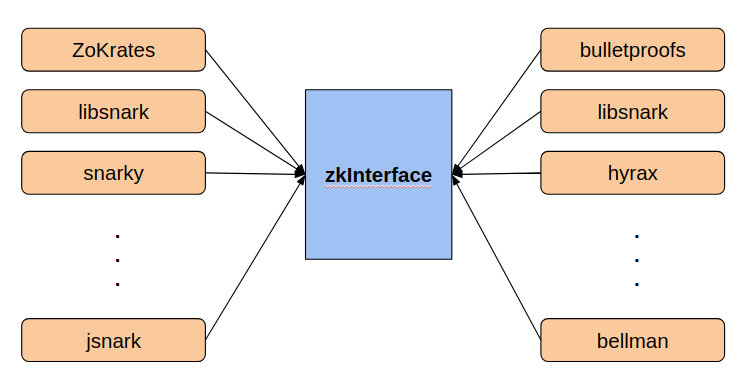
\includegraphics[width=\linewidth]{interface.png}
	\caption{zkInterface\enote{Replace by diagram on slack}}
	\label{interface}
\end{figure}

%=============================================================================
\section{Design}
\label{sec:design}

%-----------------------------------------------------------------------------
\subsection{Approach}

	zkInterface is a procedural, purely functional interface for zero-knowledge systems that enables cross-language interoperability. The current version, even if limiting, creates an interface based on R1CS formatting and offers the ability to abstractly craft a constraint system building from different gadgets, possibly written in different frameworks, by defining how data should be written and read.
	It is independent of any particular proving systems.

	The same interface can be used in two use-cases:
	\begin{itemize}
		\item To connect the construction and execution of a zero-knowledge program
			to a proving system. See Figure \ref{fig:programproving}.

		\item To decompose a zero-knowledge program into multiple gadgets that can be engineered separately. See Figure \ref{fig:programcomponents}.
	\end{itemize}
	
\begin{figure}[!h]
	\centering
	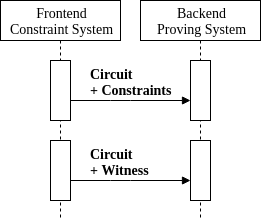
\includegraphics[width=0.5\linewidth]{graphics/program_proving.png}
	\caption{The interaction between a zero-knowledge program and a proving system.}
	\label{fig:programproving}
\end{figure}

\begin{figure}[!h]
	\centering
	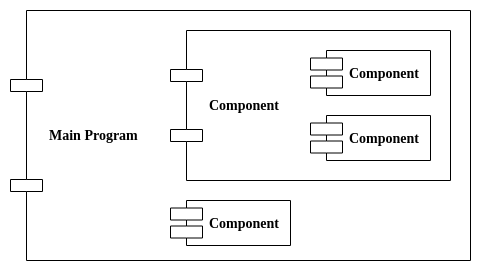
\includegraphics[width=0.7\linewidth]{graphics/program_components.png}
	\caption{A zero-knowledge program built from multiple gadgets.}
	\label{fig:programcomponents}
\end{figure}


\parhead{Interface}

	The interaction between caller and gadgets is based on exchanging messages.
	Messages are purely read-only data, which grants a great flexibility to
	implementations of gadgets and applications.

\parhead{Interoperability}

	Different parts of an application may be written in different programming languages, and interoperate through messages.
	These parts may be linked and executed in a single process, calling functions,
	and exchanging messages through buffers of shared memory.
	They may also run as separate processes, writing and reading messages in files, or through pipes or sockets.
	Some implementation strategies are discussed in section~\ref{sec:implementation}.

\parhead{Messages Definition \label{messagedefinition}}

	The set of messages is defined in Listing \ref{zkinterface.fbs},
	using the FlatBuffers interface definition language.
	All messages and fields are defined in this schema.

	The FlatBuffers system includes an interface definition language
	which implies a precise data layout at the byte level.
	Code to write and read messages can be generated for all common programming languages.
	Examples are provided for C++ and for Rust.

	Multiple paths for evolution and extensions of the standard are possible,
	thanks to the flexibility and backward-compatibility features of the encoding.
	The encoding is designed to require little to no data transformation, making it possible
	to implement the standard with minimal overhead in very large applications.

	Messages must be prefixed by the size of the message not including the prefix,
	as a 4-bytes little-endian unsigned integer.
	This makes it possible to concatenate and distinguish messages
	in streams of bytes or in files.

	The specification of FlatBuffers can be found at
	\href{https://google.github.io/flatbuffers/}{https://google.github.io/flatbuffers/}.


\parhead{Instance and Witness Reductions}

	Instance reduction is the process of constructing a constraint system.
	Witness reduction is the process of assigning values to all variables
	in the system before generating a proof about concrete input values.

	When using a proving system with pre-processing, instance reduction
	is performed once ahead of time and used in a trusted setup.
	In proving systems without pre-processing, instance reduction is used in proof verification.
	The standard supports both execution flows.


%-----------------------------------------------------------------------------
\subsection{Architecture}

\begin{figure}[!h]
	\centering
	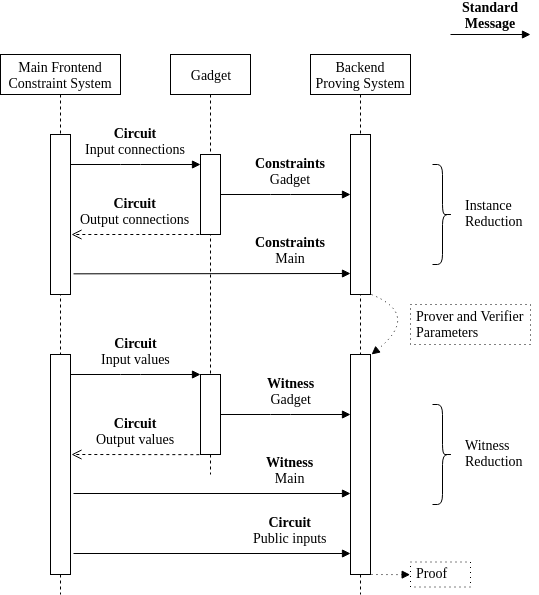
\includegraphics[width=\linewidth]{graphics/call_flow.png}
	\caption{The flow of messages between libraries using the interface.}
	\label{fig:flow}
\end{figure}

\parhead{Messages Flow}
	The flow of messages is illustrated in Figure \ref{fig:flow}.

	The caller calls the gadget code with a single \textid{GadgetCall} message.
	The gadget exits with a single \textid{GadgetReturn} message.
	This is a control flow analoguous to a function call in common programming languages.

	The caller can request an instance reduction, or a witness reduction, or both at once.
	This is controlled by the fields \textid{generate\_r1cs} and \textid{generate\_assignment} of \textid{GadgetCall} messages.

	During instance reduction,
	a gadget may add any number of constraints to the constraint system
	by sending one or more \textid{R1CSConstraints} messages.
	The caller and other gadgets may do so as well.

	During witness reduction,
	a gadget may assign values to variables
	by sending one or more \textid{AssignedVariables} messages.

\parhead{Messages Channels}
	The caller provides the gadget with the means to send messages,
	or output channels.	This can be implemented in various ways depending
	on the application.
	The caller may arrange a distinct channel for each message type,
	and the gadget must send messages to the appropriate channels.

	\noteparagraph{Note}
	This design allows a gadget to call other gadgets itself.
	All \textid{R1CSConstraints} or \textid{AssignedVariables} messages
	from all (sub-)gadgets may be sent to a shared channel
	without the need to aggregate them into a single message,
	and independently of the call/return flow.
	Moreover, an implementation can decouple the proving system
	from the logic of building constraints and assignments,
	by arranging for the constraints and assignments messages
	to be processed by the proving system, independently from the control logic.

\parhead{Variables}
	The constraint system reasons about variables, which are assigned a numerical identifier that are unique within a constraint system. The variable numbers are incrementally allocated in a global namespace. Messages that contain constraints or assignments refer to variables by this numeric ID. It is up to gadgets that create the constrain system to keep track of the semantics (and if desired, helpful symbolic names) of the variables that they deal with, and to allocate new variables for their internal use. The messages defined by the framework include a simple protocol for conveying the state of of the variable allocator (i.e., the first free variable number), and the identity of variables that tie a gadget to other gadgets.

	\noteparagraph{Note}
	This design allows implementations to aggregate and handle messages in a generic way,
	without any	reference to the gadgets or mechanisms that generated them.

\parhead{Local Variables Allocation}
	A gadget may allocate a number of local variables to use
	in the internal implementation of the function that it computes.
	They are analoguous to stack variables in common programming languages.

	The following protocol is used to allocate variable IDs that are
	unique within a whole constraint system.
	\begin{itemize}
		\item The caller must provide a numerical ID greater than all IDs that have already been allocated, called the Free-Before ID.
		\item The gadget may use the Free-Before ID and consecutive IDs as its local variables IDs.
		\item The gadget must return the next consecutive ID that it did not use, called the Free-After ID.
		\item The caller must treat IDs lesser than the Free-After ID as allocated by the gadget,
			and must not use them.
	\end{itemize}

	During instance reduction, the gadget can refer to
	its local variables in the\\
	\textid{R1CSConstraints} messages that it generates.
	The caller and other parts of the program must not refer to these local variables.

	During witness reduction, the gadget must assign values to its local variables
	by sending \textid{AssignedVariables} messages.

\parhead{Incoming/Outgoing Variables}

	The concept of incoming, outgoing variables arises when a program is decomposed into gadgets.
	These variables serve as the functional interface between a gadget and its caller.
	They are analoguous to arguments and return values of functions in common programming languages.
	A variable is not inherently incoming, outgoing, nor local;
	rather, this is a convention in the context of a gadget call.

	The caller provides the IDs of variables to be used as incoming and outgoing variables by the gadget.
	There may be no outgoing variables if the gadget implements a pure assertion.

	During instance reduction, both the caller and the gadget can refer to
	these variables in the \textid{R1CSConstraints} messages that they generate.
	Other parts of the program may also refer to these same variables in their own contexts.

	During witness reduction, the caller must pass incoming values to the gadget in the \textid{GadgetCall} message.
	The gadget must return outgoing values to the caller in the \textid{GadgetReturn} message.

	The caller is responsible for the assignment of values to both incoming and outgoing variables.
	How this is achieved depends on the caller and proving system,
	and on whether some variables are treated as public inputs of the instance.


%Rewriting \section{Description}
		
		zkInterface is a purely functional interface for zero-knowledge systems that enables cross-language interoperability via dynamic linking and shared memory. The current version, even if limiting, creates an interface based on R1CS formatting and offers the ability to abstractly craft a constraint system building from different components, possibly written in different frameworks, by determining how data should be written and read. 
		
		It can also be seen as a design tool for improved generation of constraints and usability, analogous to a portable binary format, since one can parametrize the functions calls and easily compose different functions, or components, that are not directly compatible.
		
		It is important to point out that the interface can be called both to write a request or read a response by having an encoder at the front-end  and a decoder at the back-end. 
		
		\paragraph{Main functionality.}
		
		The interface works across every zero-knowledge front-end and back-end, minimizing, when possible, the overhead of using a general format. This is achieved in several ways:
        
        \begin{itemize}
			\item By using a protoboard-like method for shared memory allocation, and thus preventing double-copying the data unnecessarily.
			\item By parametrizing the function calls to the different components so to take advantage of the specific context underlying those components.
			\item By using FlatBuffers, an efficient cross platform serialization library for different languages. This tool allows us to easily write ad-hoc parsers from scratch and has a very low overhead in shared memory, which can be used in regular function calls. 
		\end{itemize}
		
		
        
        The two main purposes of the interface are the computations of the \emph{instance reduction}, which generates a portable circuit or constraint system, and the \emph{witness reduction}, which assigns values to the variables allocated in the instance reduction. We have designed the interface so that each of these two processes actually use the same exact routine, except with different message types.

        Essentially, as seen in Figure \ref{flow}, the caller of the interface can be both an application or a component that requires a sub-component, an abstraction that helps make the interface minimal. Say I want to compute a proof of set membership by using a Merkle Tree of hashes. Then, the flow is the following:
        \begin{enumerate} 
            \item The application will call the Merkle Tree component that exists in some front-end framework, which starts allocating in memory the variables and constraints in the standard R1CS format.
            \item For every hash computation needed to generate the path, the Merkle Tree will itself call a hasher sub-component, possibly from a different framework, by passing it the parameters, including the next free memory slot for allocating the hash constraints and variables.
            \item The hash component will then allocate in memory the constraints and variables, to which the Merkle Tree component is oblivious (except the shared input / outputs: the input message and the output hash digest).
            \item Specifically, for each call to the hash component, the input message is given as part of the request and the hash component sends the hash digest as part of the response. The rest of the variables are locally dealt with by the hash component but are shared in memory by all the components.
        \end{enumerate}
        
        Note how the routine can be re-used by the witness reduction and deterministically assign the values to the respective variables in memory. Moreover, if needed, the constraint system can be outputed as a file containing a static rank-1 constraint system. One objection to using this routine design is that the component at the top level (i.e.: the Merkle Tree) cannot is waiting for the response of the sub-component (i.e.: the hasher component). This can have a cost in the efficiency of the circuit generation if we imagine a long enough chain of sub-calls that would cause a quadratic overhead. This is unlikely to happen in the current set of applications and circuits. \dtodo{Please check that this is true}
		
			\begin{figure}[h!]
				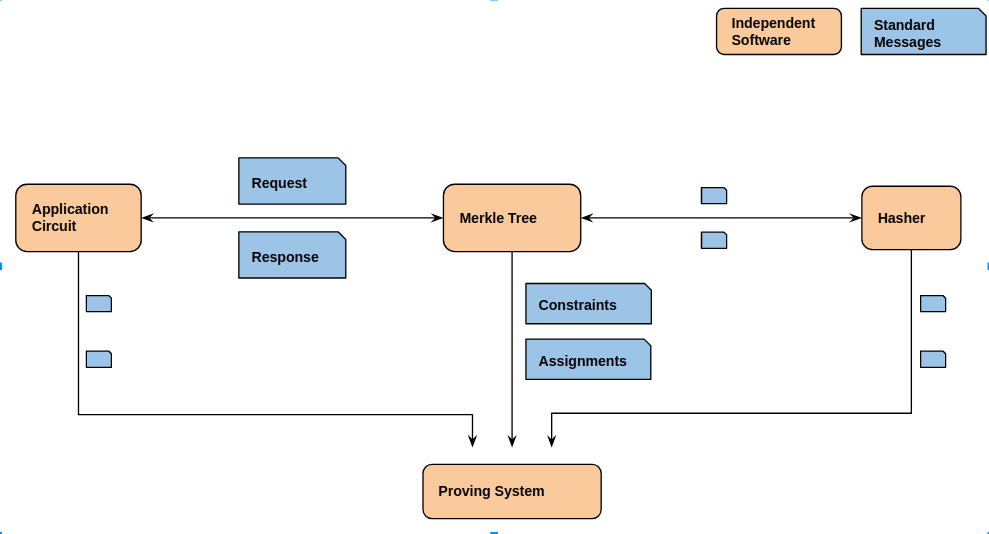
\includegraphics[width=\linewidth]{routine.png}
				\caption{The flow of interaction between existing libraries and the interface}
				\label{flow}
			\end{figure}

		\paragraph{Instance reduction.} 
		
        Points to include:
        - caller does not provide functionality to gadget and does not depend on specific implementation
        - gadget and caller both allocate variables
		
		\paragraph{Witness reduction.}
		
		r1cs in the format: a way to represent the constraints and a way to represent the assignment; and connection between components (gadgets), which actually are the public inputs. If we think of circuit as components, each component has a set of local inputs and "outgoing" inputs.
		
		So the interface solves two problems: 1/ interop between frameworks (front-ends) and proving systems (backends) 2/ composability of gadgets between different frameworks.
		
	
		
		\subsection{An MVP}
		
		
		
		\subsection{Specification}
        
        \paragraph{Interface Definition.}
        
        \paragraph{Request Call.}

        \paragraph{Callee Response.}

        \paragraph{Memory Allocation.}

        \paragraph{FlatBuffers.}

        \paragraph{Standard Format.}

		*use of flatboard
		
		- semantics; planned parametrization of the semantics.
		
		- format: can work with files (all messages instead of processing, can be written to file) for both instance / witness reduction, otherwise can work with memory 
		
		Each component has an interface; which can be invoked / instantiated / called with other components to make up the constraint system.
			- composibility of gadgets as there local variables / public ones (merkle tree has the leaf and root and invokes sha256)
		
		CRS is specific to proving system so the format does not handle the CRS portability
		
		we are thinking of implementing ZoKrates for the application layer and libsnark, bellman.  
		
		NOTE: some people think of functions, inputs and returned variables; others as circuits and gadgets.
		
		
		Issues: 1/ linear 

\subsection{Interface Definition}

	\lstinputlisting[
		caption=gadget.fbs - Interface definition,
		language=flatbuffers2,style=protobuf,
		label=gadget.fbs]{../gadget.fbs}

	\lstinputlisting[
		caption=gadget.h - C Interface,
		language=C++,style=protobuf,
		label=gadget.h]{../cpp/gadget.h}

\end{document}